\chapter{Grundlagen}

\section{Google Design Sprint}

Der Google Design Sprint \ac{GDS} ist eine von Jake Knapp bei Google Ventures entwickelte Methodik zur schnellen und effizienten Problemlösung sowie Produktentwicklung, insbesondere für Herausforderungen, die sich aus der dynamischen Natur des Marktes und den sich verändernden Produktanforderungen ergeben. 
Ziel dieser Methode ist es, innerhalb eines Zeitraums von fünf Tagen einen Prototyp zu entwickeln und zu evaluieren. 
Diese Methode bietet den Vorteil, dass nicht auf die Markteinführung gewartet werden muss, um Feedback zu erhalten. Stattdessen können dringende Fragen sofort beantwortet werden \cite[S.98 f.]{Design_Sprint}.

Die fünftägige Methode, wie in Abbildung \ref{GDS} dargestellt, verläuft wie folgt:

\begin{figure}[h]
    \centering
    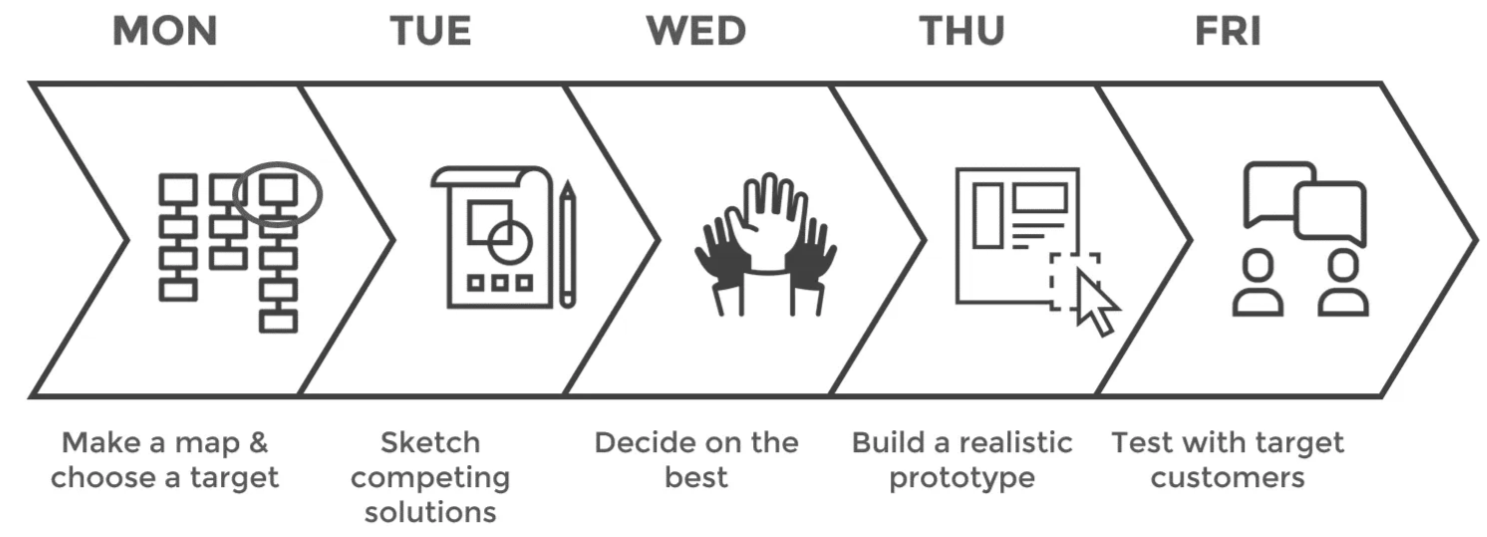
\includegraphics[clip,width=0.75\linewidth]{images/GDS.png}
    \caption[Ablauf eines GDS]{Ablauf eines GDS \cite{GDS_Abbildung}}
    \label{GDS}
\end{figure}

Am ersten Tag geht es darum, das Problem zu verstehen und den Fokus für die Woche festzulegen. Das Team definiert das langfristige Ziel und identifiziert die Herausforderung. 

Am zweiten Tag konzentriert sich das Team auf die Bewältigung bereits bekannter Herausforderungen. Anders als bei herkömmlichen Brainstorming-Sitzungen arbeiten die Teammitglieder einzeln an Lösungsansätzen und folgen einem strukturierten vierstufigen Prozess, um das kritische Denken zu fördern. 

Am dritten Tag trifft das Team Entscheidungen darüber, welche Idee als Prototyp entwickelt und getestet werden sollen. Dabei kommt die fünfstufige "Sticky Decision"-Methode zum Einsatz, um die besten Lösungen zu identifizieren. Anschließend wird ein detaillierter Prozessplan für den Prototypen erstellt. 

Am vierten Tag wird ein realitätsnaher Prototyp entwickelt. Das Ziel ist es, eine testbare Version der Lösung zu erstellen, die am nächsten Tag mit echten Nutzern evaluiert werden kann. 

Der letzte Tag ist für das Testen des Prototyps reserviert. Das Team sammelt Feedback von echten Nutzern und erhält Einsicht, ob die Lösung in der Praxis funktioniert und welche Anpassungen nötig sind. Dieses Feedback ist entscheidend, um die Stärken und Schwächen der entwickelten Lösung zu identifizieren \cite[S.22 ff.]{Design_Sprint}.

\section{User Experience}
Das Design der User Experience \ac{UX} konzentriert sich auf jedes Element und jede Funktion, die der Benutzer bei einer Anwendung sieht, mit dem Ziel, eine möglichst angenehme und effiziente Erfahrung zu ermöglichen \cite[S.12]{Bordegoni}. 
Laut der International Organization for Standardization (ISO 9241-210) wird UX definiert als „Wahrnehmungen und Reaktionen einer Person, die sich aus der Verwendung und/oder der erwarteten Verwendung eines Produkts, Systems oder einer Dienstleistung ergeben” \cite{iso}. 
Während sich das User Interface auf das Erscheinungsbild der Anwendung konzentriert, beispielsweise auf Schriftarten und Farben, geht die UX tiefer und umfasst das gesamte Erlebnis des Nutzers \cite[S.8]{Canziba}.

In den letzten Jahrzehnten hat die Bedeutung der User Experience stark zugenommen, da Unternehmen erkannt haben, dass ein positives Nutzungserlebnis entscheidend für den Erfolg eines Produkts ist \cite{ux_article}. 
Bei einem schlechten UX-Design fällt es den Benutzern schwer, die Anwendung zu nutzen, und sie wechseln, sobald sie eine ähnliche, bessere App gefunden haben, die die gleiche Aufgabe erfüllt. 
Deshalb ist es für ein gutes UX-Design wichtig, dass der Designer die Bedürfnisse der Benutzer vorhersieht und erfüllt, indem er ihre Sichtweise einnimmt. Ein gutes UX-Design kann die Produktivität steigern, die Zufriedenheit der Kunden erhöhen und die Verkaufszahlen verbessern. 
Zudem können durch eine optimierte Benutzererfahrung die Kosten für Support und Wartung gesenkt werden \cite[S.8 ff.]{Canziba}.

Die UX umfasst verschiedene Komponenten, die zusammenarbeiten, um ein positives Nutzungserlebnis zu schaffen. Dazu gehören Usability, Ästhetik, Interaktion und Emotionalität.

Die Usability bezieht sich auf die Benutzerfreundlichkeit und Effizienz eines Produkts. 
Ein System mit hoher Usability ermöglicht es den Nutzern, ihre Ziele schnell und ohne Frustration zu erreichen. 
Dies beinhaltet Aspekte wie Lernfähigkeit, Effizienz der Nutzung und Zufriedenheit der Nutzer \cite[S.23 ff.]{Nielsen}.

Die Ästhetik bezieht sich auf das Erscheinungsbild des Produkts.   
Ein ansprechendes visuelles Design kann die Wahrnehmung der Qualität und den Gesamteindruck eines Produkts erheblich verbessern. 
Studien zeigen, dass ästhetisch ansprechende Designs oft als funktionaler und benutzerfreundlicher wahrgenommen werden \cite{Tractinsky}.